\documentclass{article}
\usepackage{minted}
\usepackage{braket}
\usepackage{graphicx}

\title{The Journey of Building \\ \underline{Qubit Simulator}}
\author{Brian Hernandez}
\date{Latest Update: June 17, 2026}

\begin{document}

\maketitle

\section{Introduction}

This document chronicles my journey in creating \textbf{Qubit Simulator}. It captures my thought process, all my fails, successes, and ideas for the future to come. 

\section{The Language}

Since finding the probability amplitudes of a qubit without explicit calculation is impossible, it is necessary to use matrix multiplication to find the state after each operation applied. While I could use Python or a library that already implements matrix multiplication, what's the fun in that?\newline{}
So the first step is to make a library that implements matrix multiplication, and what better language to do it in than C?
It's fast, simple, and straightforward. It has all I need: no more, no less\dots
Or so I thought. I realized shortly after writing my first few classes that using WebAssembly would be too tedious and using HTTP server communication would over-complicate this app for no reason. 
So I did what I least wanted to do: I scrapped using C and resorted to writing everything in Typescript instead.


\section{The Clases}
\subsection{Complex Numbers}
So with the language choice out of the way, we can start implementing some linear algebra: The first step is to use a class to implement complex numbers. It simply has to have a real part and imaginary part:
\\
\begin{minted}{typescript}
    export class ComplexNumber 
    {
        realPart : number;
        imaginaryPart : number;

        constructor(realPart : number, imaginaryPart : number) 
        {
            this.realPart = realPart;
            this.imaginaryPart = imaginaryPart;
        }
    }
\end{minted}

\subsection{Vectors, Bras, and Kets}
By the Fundamental Postulate, any quantum system can be completely described by a state vector, which is a unit vector containing the amplitudes for each orthogonal state.\footnote{Cottrell, Seth \textit{Quantum Computation: An Introduction for Undergraduates, page 39}}
Since we are dealing with qubits, we technically only need a 2-element vector to hold \(\alpha\) and \(\beta\). 
However, this is mainly an educational app, so might as well take the opportunity to implement a general vector system that can accomadate any number of orthogonal states and just have a qubit be an implementation of a 2-state vector.
Here's the general vector: 
\begin{minted}{typescript}
export class AmplitudeVector
{
    complexNumbers : ComplexNumber[];
    length : number;

    constructor(complexNumbers: ComplexNumber[])
    {
        this.complexNumbers = complexNumbers;
        this.length = complexNumbers.length;
    }

    
}
\end{minted}
Each element is a complex number because each probability ampltitude associated with an orthogonal state is a complex number.\\
\\
Now a state vector can take one of two forms: A Bra or a Ket:
\begin{minted}{typescript}
    export class Bra extends AmplitudeVector 
    {
        constructor(complexNumbers: ComplexNumber[])
        {
            super(complexNumbers);
        }

        conjugateTranspose() : Ket
        {
            let complexNumbers = [];
            for (let i = 0; i < this.length; i++)
            {
                complexNumbers.push(this[i]);//copy
                complexNumbers[i].imaginaryPart *= -1;//flip sign
            }

            return new Ket(complexNumbers);
        }

    }

    export class Ket extends AmplitudeVector 
    {
        constructor(complexNumbers: ComplexNumber[])
        {
            super(complexNumbers);
        }

        conjugateTranspose() : Bra
        {
            let complexNumbers = [];
            for (let i = 0; i < this.length; i++)
            {
                complexNumbers.push(this[i]);//copy
                complexNumbers[i].imaginaryPart *= -1;//flip sign
            }

            return new Bra(complexNumbers);
        }
    }
\end{minted}

Notice that these classes each have a conjugateTranspose() function. This is what transforms a Bra to a Ket and vice-versa. When it is applied to a state vector, it is as if a dagger (\(\dagger\)) were applied to it:
\[
\ket{\psi}^{\dagger} = \bra{\psi}
\]
\[
\bra{\psi}^{\dagger} = \ket{\psi}
\]
The conjugate transpose or "dagger" turns a row vector into a column vector and vice versa, and flips the sing of the imaginary part of each element. This flipping of the imaginary part's sign is also known as taking its "complex conjugate" or the \(*\) operation: \(\alpha^*  =  a  - bi\)
\\
\subsection{Qubits}
Now that we have our bras and kets, we can implement the two-state implementation of each of these: the qubit.
A qubit is simply a two-element vector (bra or ket) where we call the probability amplitude of the first element alpha: \(\alpha\) and the probability amplitude of the second element beta: \(\beta\) for simplicity. 
The first element probability amplitude corresponds to some state, usually 0 from the computational basis, and the second element probability amplitude corresponds to the state orthogonal to the first element's state — in the case of the computational basis, this is 1. 
These two states make up a \textbf{basis}.

From these probability amplitudes, we can derive the most important aspects of a qubit in this current situation: \( \theta \) and \( \phi \).
The main idea is this: Any qubit can be represented in the following form: \[\ket{\psi} =  \cos(\frac{\theta}{2}) + e^{i\phi}\sin(\frac{\theta}{2})\]
where \(\theta\) is the angle formed between the positive z axis and the position of the qubit on the bloch sphere, and \(\phi\) is the azimuthal angle formed between the positive x axis and the qubit on the bloch sphere:

\begin{figure}[h]
    \centering
    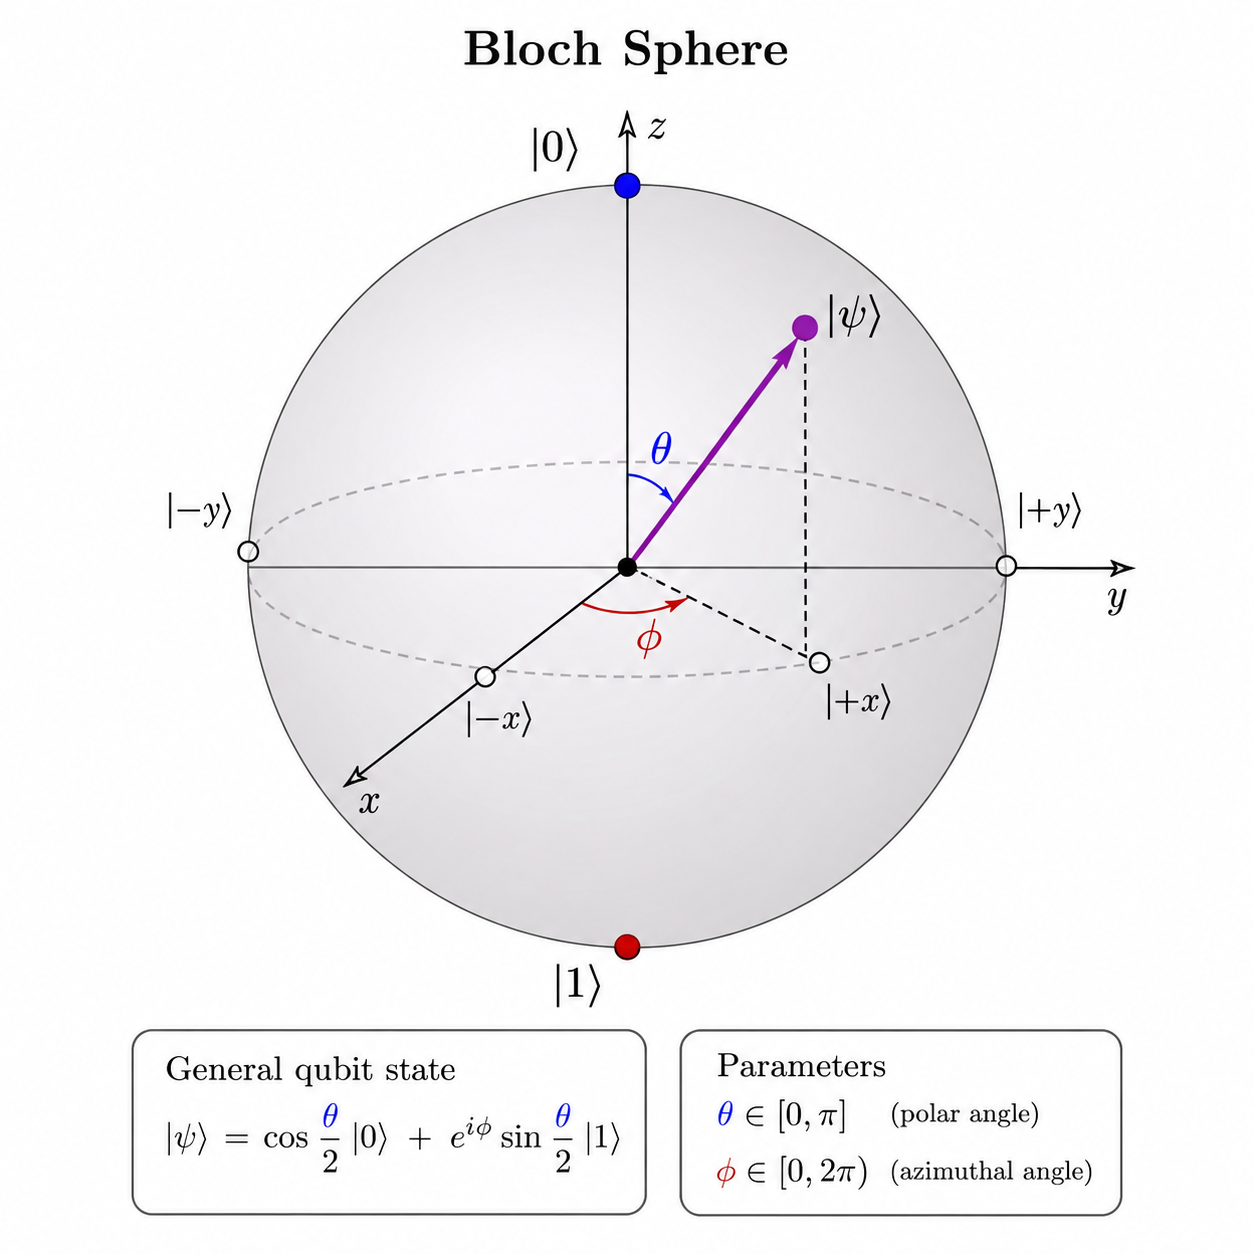
\includegraphics[width=0.7\textwidth]{./journey_images/bloch_sphere.png}
    \caption{The Bloch sphere \protect\footnotemark}
    \label{fig:bloch-sphere}
\end{figure}
\footnotetext{Figure generated by ChatGPT.}

\end{document}